\documentclass[12pt]{article}
\usepackage{amsmath}
\usepackage{graphicx}
\usepackage{caption}
\usepackage{subcaption}
\usepackage{booktabs}
\usepackage{float}
\usepackage[utf8]{inputenc}
\usepackage{geometry}
\usepackage{multirow}
\usepackage{setspace}
\usepackage{parskip}
\usepackage{svg}
\usepackage[bottom]{footmisc}
\usepackage{tikz}
\usepackage[section]{placeins}

% This style is used to create block diagrams, you'll find it useful since many of your figures would be of that form, I'll try add more styles in the future :)
\usetikzlibrary{trees,positioning,fit,calc}
\tikzset{block/.style = {draw, fill=blue!20, rectangle,
                         minimum height=3em, minimum width=4em},
        input/.style = {coordinate},
        output/.style = {coordinate}
}

\usepackage[section]{minted}
\usepackage{xcolor}
\usemintedstyle{porland}

\usepackage{chngcntr}
\counterwithin{figure}{section}

\renewcommand{\arraystretch}{1.5}

\usepackage[hidelinks]{hyperref}
\hypersetup{
    linktoc=all
}

\renewcommand\listingscaption{Listing}
\renewcommand\listoflistingscaption{List of Listings}

\usepackage{scrhack}
\usepackage{tocbasic}
\setuptoc{lol}{levelup}

\usepackage{indentfirst}
\geometry{a4paper, margin=1in}

%------------------------------------------------%

\setlength{\parindent}{0em}
\setlength{\parskip}{0em}

\begin{document}

\begin{center}
 	{\Huge Sección 3}\\
	 \vspace{0.75cm}
	 {\large Probabilidad y Estadística ejercicios}\\
	 \vspace{0.5cm}
\end{center}
{\large Daniela Jijón, Juan Francisco Cisneros y Luciana Valdivieso}\\
\vspace{0.5cm}
{\large24 de julio de 2022}\\

\pagenumbering{Roman}
\setlength{\parskip}{\baselineskip}%

\pagenumbering{arabic}

%--------------SECCIONES ---------------------%

\section{Estadística Inferencial}
\subsection{Intervalos de Confianza}

Intervalos de confianza para la media de las variables cuantitativas con un nivel de confianza del 99\%

\begin{equation}
	\=x - Z _{\alpha/2}\frac{\sigma}{\sqrt[]{n}}>\mu <  \=x + Z _{\alpha/2}\frac{\sigma}{\sqrt[]{n}}\\
\end{equation}
\begin{align*}
    &Z _{\alpha/2} = 2.57
\end{align*}

Variable GPA
\begin{align*}
    & 2.42 >\mu <  4.52
\end{align*}

Variable Horas de Estudio Semanales
\begin{align*}
    & -6.04>\mu < 30.47
\end{align*}

Variable Año
\begin{align*}
    & -0.683 >\mu <  5.357
\end{align*}

Variable Edad
\begin{align*}
    &14.93 >\mu < 24.525
\end{align*}

\clearpage

\subsection{Hipótesis}
\begin{align*}
    & H_{o}: \mu_{mujeres} - \mu_{hombres} = 0 \\
    & H_{a}: \mu_{mujeres} - \mu_{hombres} > 0 \\
\end{align*}

Estadístico:
\begin{align}
    &Z = \frac{\=x -\=y}{S_{\=x -\=y}}
\end{align}
\begin{align*}
    &Z = 49.348
\end{align*}
\begin{align*}
    valor P &= 0
\end{align*}

El valor P tiende a cero, no se rechaza la hipótesis nula. Para los niveles de confianza $0.05, 0.01, 0.001$ se obtiene que no se rechaza la hipótesis nula ya que $Z \geq Z_{\alpha}$

\begin{align}
    F & = \frac{S_{mujeres}{S_{hombres}}
\end{align}
\begin{align*}
    F & = 0.9154
\end{align*}

Valores críticos de F:
\begin{align}
    I & = f_{1- \alpha/2, \nu_{1}, \nu_{2}}\\
    D & = f_{\alpha/2, \nu_{1}, \nu_{2}}
\end{align}

\begin{align*}
    f_{0.025, 98, 101} & = 0.6739\\
    f_{0.975, 98, 101} & = 1.4839\\
\end{align*}

No hay evidencia de diferencia significativa de las varianzas en ambas variables de GPA

\clearpage

\section{Regresión Lineal}
Variable independiente: Horas de estudio de semanales\\
Variable dependiente: GPA\\
\begin{equation}
	\hat y = \hat\beta_{o} + \hat\beta_{1} x
\end{equation}
\begin{align*}
    \hat\beta_{o}& = \=y - \hat\beta_{1}\=x\\
    \hat\beta_{1}& =  \frac{SCxy}{Sxx}
\end{align*}
\begin{align*}
    SCxy& =  130.69
\end{align*}
\begin{align*}
    Sxx& =  9905.42
\end{align*}
Obtenemos:\\
\begin{align*}
    \hat\beta_{o}&=3.306\\
    \hat\beta_{1}&=0.0132\\
    \hat y&= 3.306 +  0.0132x
\end{align*}


Existe buen ajuste pero no es significativo

Suma de Errores y $r^{2}$:
\begin{align}
    SCE &=SCy - \hat\beta_{1}SCxy\\
    r_{xy}&=\frac{SCxy}{\sqrt[]{SCx \cdot SCy}}
\end{align}

\begin{align*}
    SCE &= 30.93\\
\end{align*}
\begin{align*}
    r^{2}&=r_{xy}^{2}\\
    r^{2}&= 0.0528\\
\end{align*}

Intervalo de confianza Coeficiente de Correlación:

\begin{align*}
    Z_{r}& = \frac{ln(\frac{1+r}{1-r})}{2}\\
    Z_{r}& = 0.234   
\end{align*}

\begin{equation}
	Z _{r}-\frac{Z _{1-\alpha/2}}{\sqrt[]{n-3}}> r < Z _{r}+\frac{Z _{1-\alpha/2}}{\sqrt[]{n-3}} \\
\end{equation}
\begin{equation*}
	0.095 > r < 0.3729\\
\end{equation*}

El intervalo contiene 0

Al realizar los cálculos con paquetes de python hemos obtenido los mismos resultados que de manera algebráica\\
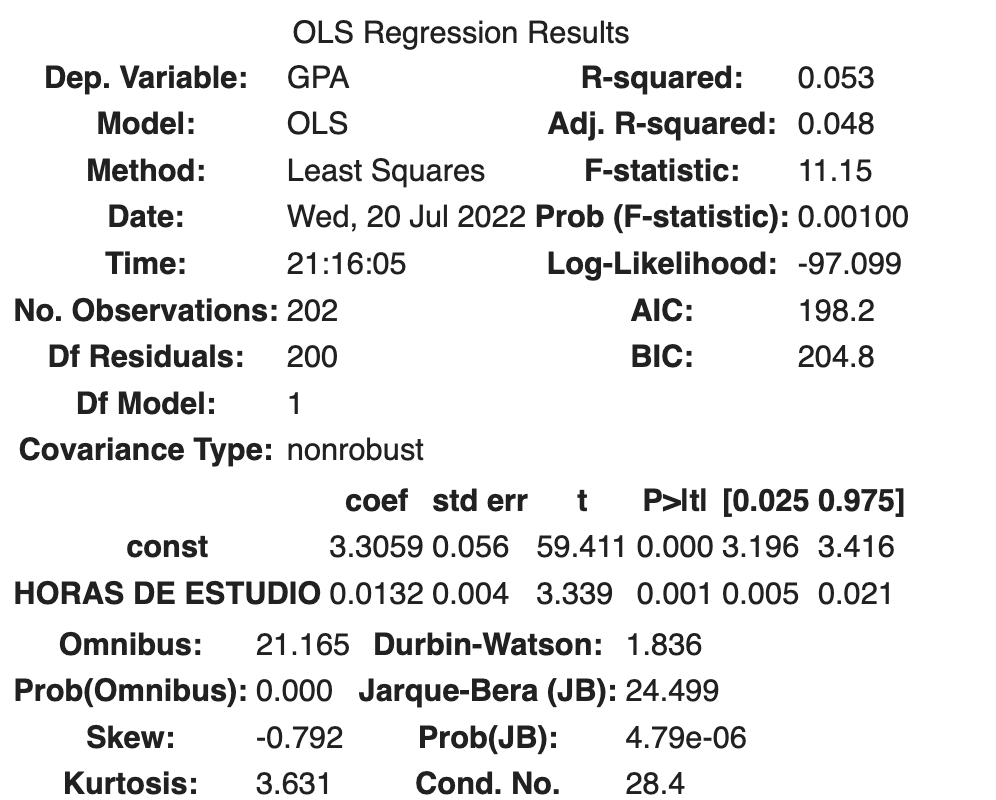
\includegraphics[width=8cm, height=7cm]{resultados}

Gráfico de Correlación\\
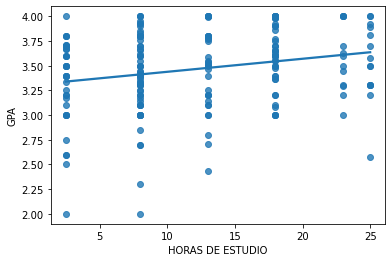
\includegraphics[width=8cm, height=7cm]{regresion}
\end{document}